\documentclass[12pt,a4paper,oneside]{report}
\usepackage[brazil]{babel}
%\usepackage[portuges]{babel}
\usepackage[T1]{fontenc}
\hyphenation{li-vro tes-te cha-ve bi-blio-te-ca}
\hyphenation{co-men-t-rio re-fe-rn-cia}
\usepackage[utf8x]{inputenc}
\usepackage[pdftex]{graphicx}
\usepackage{epstopdf}
\DeclareGraphicsRule{.tif}{png}{.png}{`convert #1 `dirname #1`/`basename #1 .tif`.png}
\usepackage{amsmath}
\usepackage{amssymb,amsfonts,textcomp}
\usepackage{array}
\usepackage{hhline}
\usepackage{subfig}
\author{Bruno Lima Cardoso}
\linespread{1.5}
\usepackage{indentfirst}
\pagestyle{plain}
%\pagestyle{empty}
\usepackage{hyperref}
\hypersetup{
    colorlinks,%
    citecolor=blue,%
    filecolor=black,%
    linkcolor=black,%
    urlcolor=blue
}

%\title{T\'itulo do Trabalho}

\begin{document}

%%%%%%%%%%%%%%%%%%%
% parte frontal
%%%%%%%%%%%%%%%%%%%
\begin{titlepage}
\clearpage
\bigskip


\bigskip



\bigskip

\centerline{\textbf{\large \emph{Web of Things:} Uma Prova de Conceito com Aplicação em Acessibilidade}}


\bigskip


\bigskip

\centerline{\textbf{Bruno Lima Cardoso}}



\bigskip


\bigskip

Projeto Final de Curso submetido ao Departamento de Ci\^encia da Computa\c{c}\~ao do Instituto de Matem\'atica da Universidade Federal do Rio de Janeiro como parte dos requisitos necess\'arios para obten\c{c}\~ao do grau de Bacharel em Ciêcia da Computação.


\bigskip

Apresentado por: Bruno Lima Cardoso


\bigskip


%\hfill
%\_\_\_\_\_\_\_\_\_\_\_\_\_\_\_\_\_\_\_\_\_\_\_\_\_\_\_\_\_
\hfill
\line(1,0){250}

\hfill
Bruno Lima Cardoso

\bigskip

\hfil
Aprovado por:

\bigskip

\bigskip

\hfill
\line(1,0){250}

\hfill
Prof. Gabriel P. Silva, D. Sc.

\hfill
(Presidente)

\bigskip

\bigskip

\bigskip

\hfill
\line(1,0){250}

\hfill
Prof. José Antonio Borges, D. Sc.

\bigskip

\bigskip

\bigskip

\hfill
\line(1,0){250} 

\hfill
Prof. Fernando Gil Vianna Resende Junior, Ph. D.

\bigskip

\bigskip

\bigskip

\bigskip

\begin{center}

RIO DE JANEIRO, RJ - BRASIL

AGOSTO DE 2012

\end{center}

\bigskip

\clearpage
\bigskip

\begin{center}
\centerline{\textbf{\large RESUMO}}


\bigskip

\emph{Web of Things:} Uma Prova de Conceito com Aplicação em Acessibilidade


\bigskip

Bruno Lima Cardoso


\end{center}
\bigskip


\bigskip


Orientador: Gabriel P. Silva 


\bigskip


\bigskip

Este trabalho apresenta um sistema que propicia maior independência funcional aos portadores de lesão motora severa, para que dispensem o auxílio de terceiros para interagir com o ambiente ao seu redor. Para tal, foi desenvolvido um protótipo de um sistema de automação residencial cujo objetivo é virtualizar o acesso a aparelhos eletrônicos como, televisão, sistema de som e similares,  possibilitando que o deficiente os acesse diretamente. Utilizando Web of Things como arquitetura base, será mostrado que este conceito é possível e extremamente viável. O protótipo desenvolvido possui três camadas: rede de sensores e atuadores (virtualizador dos aparelhos), o Smart Gateway (que padroniza o acesso aos aparelhos) e a aplicação (um controlador pertencente ao usuário). Nesta última camada em especial, será apresentada uma implementação de uma tecnologia amplamente utilizada para acessibilidade virtual, e que está em franco crescimento: o reconhecimento de voz. Ao final, serão discutidas algumas peculiaridades do protótipo apresentado, tais como, curva de aprendizagem, grau de complexidade de desenvolvimento e abordagens tomadas que poderiam ser melhoradas. Provar o conteúdo teórico apresentado aqui está além do escopo deste projeto, mas espera-se que o trabalho apresentado sirva de base para futuros desenvolvimentos e gere novas discussões sobre a arquitetura, o sistema e suas diversas aplicações.

\bigskip

\clearpage
\bigskip

\begin{center}
\centerline{\textbf{\large ABSTRACT}}


\bigskip

\emph{Web of Things:} Uma Prova de Conceito com Aplicação em Acessibilidade


\bigskip

Bruno Lima Cardoso


\end{center}
\bigskip


\bigskip

Supervisor: Gabriel P. Silva


\bigskip

\ \ Text that presents an abstract of the work giving a general description.


\bigskip


\bigskip


\bigskip
\end{titlepage}


\chapter*{Siglas}
\begin{list}{$\bullet$}{}
  \item[] HMM - Hidden Markov Models
  \item[] ASR – Automatic Speech Recognition
  \item[] CSR – Continuous Speech Recognition
  \item[] MFCC – Mel-Frequency Cepstral Coefficients
  \item[] CMN – Cepstral Mean Normalization
  \item[] FDP – Função Densidade de Probabilidade
  \item[] HTTP - Hypertext Transfer Protocol
  \item[] Web - World Wide Web
  \item[] REST - Representational State Transfer
  \item[] XML - Extensible Markup Language
  \item[] YAML - Yet Another Markup Language
  \item[] JSON - Javascript Object Notation
  \item[] SOAP - Simple Object Access Protocol
  \item[] RASSF - Rede de Atuadores e Sensores Sem Fio
  \item[] IP - Internet Protocol
  \item[] WoT - Web of Things
  \item[] PCD - Pessoa Com Deficiência
  \item[] PSD - Pessoa Sem Deficiência
\end{list}

\chapter*{Lista de Variáveis}
\begin{list}{$\bullet$}{}
\item[] t - unidade de tempo
\item[] $x_{t}$ - vetor de parâmetros calculado a partir de um segmento de fala
\item[] $c_{t}$- vetor de MFCCs calculado a partir de um segmento de fala
\item[] $c_{t}$ - vetor de MFFCs delta de primeira ordem computados a partir dos coeficientes $c_{t}$
\item[] $\Delta\Delta c_{t}$ - vetor de MFFCs delta de segunda ordem computados a partir dos coeficientes $\Delta c_{t}$
\item[] $\Theta$ - tamanho da janela usada para cálculo dos coeficientes delta de primeira e segunda ordens
\item[] M - um modelo oculto de Markov
\item[] X - sequência de vetores acústicos
\item[] $A = a_{ij}$ - matriz de todas as probabilidades de transição entre um estado i e outro j
\item[] $B = b_{i}$ - matriz de todas as probabilidades de emissão de saída em um determinado estado i
\item[] $\prod = \prod_{i}$ - matriz com as probabilidades de um modelo ser iniciado a partir de um estado i
\item[] S - sequência de estados
\item[] W - sequência de palavras
\end{list}

\tableofcontents

\listoffigures

\listoftables

%%%%%%%%%%%%%%%%%%%
%  parte principal
%%%%%%%%%%%%%%%%%%%

\chapter{Introdução}

Hoje em dia, a informática como um todo tem estado cada vez mais presente no cotidiano das pessoas. Isto se dá pela diminuição do custo de diversos dispositivos eletrônicos e computacionais, assim como pelo aumento das facilidades proporcionadas pelos mesmos. Tais facilidades, além de promoverem uma maior comodidade e praticidade ao público geral, se bem empregados, propiciam uma melhor qualidade de vida e independência funcional aos portadores de necessidades especiais (Pessoas com Deficiência – PCD). Como por exemplo, leitores de tela para cegos, sistemas que utilizam reconhecimento de voz para usuários que não possuem movimentos em seus membros e muitos outros.

Um exemplo de sucesso na integração entre componentes com arquiteturas, hardware e software, completamente diferentes é a internet. Nessa estrutura, aparelhos espalhados ao redor do mundo podem interagir sem nem mesmo se conhecerem um ao outro. Baseado neste princípio surge a \emph{Internet of Things}\cite{IoT} que tem explorado o desenvolvimento de aplicativos para dispositivos com o intuito de integrá-los ao mundo virtual. Desta forma, todos os objetos que possuam reforço digital adequado passariam a ser ``visíveis'' na rede. Porém, apenas posicioná-los na rede não é suficiente, é preciso que estes sejam integrados à web, na camada de aplicação, daí vem o conceito da \emph{Web of Things} \cite{wotdovad}, que é colocado como um refinamento da \emph{Internet of Things}, nesta estrutura os dispositivos tornam-se parte de um ambiente em que cada um fornece múltiplas aplicações/serviços diversificados a outros diferentes em hardware e software igualmente integrados.

O objetivo do sistema proposto neste trabalho é promover a independência funcional de portadores de lesão severas, como tetraplégicos, portadores de ELA (Esclerose Lateral Amiotrófica) e afins, permitindo a utilização de determinados aparelhos eletroeletrônicos. A solução aqui proposta consiste em virtualizar o acesso a esses aparelhos, de modo que possam ser controlados e gerenciados remotamente. Entretanto, esses aparelhos, em sua grande maioria, formam diversas pequenas ilhas de incompatibilidade. Isto ocorre devido à falta de padronização de seus protocolos e, apesar de alguns possuírem acesso à internet, o fato de não poderem ser controlados ou monitorados com a presença de programas não proprietários, tornam ainda mais difícil esse objetivo.

A proposta central deste trabalho é  de um sistema que confira independência funcional a PCDs fazendo uso da arquitetura \emph{Web of Things} para o desenvolvimento de um ambiente inteligente - \emph{Smart Building}. Seguindo esses preceitos e sem perdas de generalidade, objetivou-se desenvolver uma estrutura que permita ao usuário controlar um aparelho televisor utilizando apenas a sua voz. Para tal foi necessário:
\begin{itemize}
\item A implementação de um sistema de reconhecimento da fala para um \emph{Smartphone Android 3.2} para o reconhecimento dos comandos feitos pelo usuário.
\item A implementação de um cliente Hypertext Transfer Protocol (HTTP) em um \emph{Smartphone Android 3.2} utilizado para fazer as requisição dos recursos disponíveis.\footnote{Recursos disponíveis - referem-se as ações que podem ser executadas pelos atuadores disponíveis}
\item A implementação de um \emph{Smart Gateway (SG)} responsável por disponibilizar os recursos existentes através da Web.
\item A implementação do atuador responsável por executar as requisições feitas pelo usuário.
\end{itemize}

Este trabalho está organizado da seguinte maneira: o Capítulo \ref{chap:fundamentos} apresenta todos os fundamentos necessários para o desenvolvimento de cada estrutura integrante de um \emph{Smart Building} com arquitetura \emph{Web of Things}, além dos conceitos que envolvem um sistema de reconhecimento de fala, incluindo as etapas de treinamento dos modelos - acústicos e linguísticos - e a etapa de decodificação. O Capítulo \ref{chap:funcionamento} detalha a implementação de cada um dos componentes desenvolvidos neste projeto. O Capítulo \ref{chap:trabalhos-correlatos} apresenta os trabalhos que serviram de base e inspiração para este projeto. E por fim, o Capítulo \ref{chap:conclusao} mostra os resultados alcançados e propõe modificações futuras e possíveis expansões.

\chapter{Fundamentos}
\label{chap:fundamentos}

Neste capítulo serão apresentados os principais fundamentos que envolvem a implementação de um \emph{Smart Building} que possui \emph{Web of Things} como arquitetura base, assim como uma breve descrição das ferramentas utilizadas, como forma de facilitar o entendimento dos próximos capítulos.

Na Seção 2.1, o conceito de \emph{Web of Things} será brevemente apresentado e as estruturas possíveis para implantação do mesmo.

Nas Seções 2.2 e 2.3, os fundamentos referentes à camada de interação com o usuário serão vistos e distribuídos da seguinte forma:
\begin{itemize}
    \item Na Seção 2.2, o sistema operacional Android será apresentado de modo a justificar sua escolha, ressaltando pontos positivos e negativos que foram ponderados.
    \item Na Seção 2.3, as etapas que envolvem um Sistema de Reconhecimento de Palavras Isoladas são brevemente descritas e apresentadas em forma de diagrama. Nas subseções que seguem, os conceitos que envolvem cada etapa do sistema são apresentados de forma mais detalhada.
\end{itemize}

E, por fim, na Seção 2.4, o microcontrolador Arduino será visto, pois este foi utilizado na implementação da interface entre o sistema e o mundo físico.

%
% BASE DA ARQUITETURA - Visão geral do sistema
%
\section{\emph{Web of Things} - WoT}

A realização da \emph{Web of Things} requer a extensão da Web existente para que os objetos do mundo real e dispositivos embarcados possam interagir com ela. Entretanto, muitos destes dispositivos, apesar de possuírem microcontroladores, não conseguem conectar-se à Web, seja por limitações de \emph{hardware} (p. ex.: não possuem uma placa Ethernet) ou de \emph{software}. Para contornar este problema é possível utilizar uma rede de sensores/atuadores onde cada um destes supre as carências específicas de cada aparelho, consequentemente possibilitando sua integração e interação.

Ao invés de utilizar os protocolos Web apenas para transporte de dados, comumente utilizado em \emph{Web Services}, pretende-se fazer os dispositivos uma parte integral da mesma, usando o protocolo HTTP na camada de aplicação. Desta forma, as funcionalidades dos dispositivos do mundo real são disponíveis através da \emph{API RESTful} \cite{restws} sobre HTTP, como apresentado a seguir.

\subsection{Nós como Recursos RESTful}

O termo \emph{Representational State Transfer} (REST)\cite{w3curi} se referia, originalmente, a um conjunto de princípios de arquitetura. Na atualidade se usa no sentido mais amplo para descrever qualquer interface web simples que utiliza \emph{Extensible Markup Language} (XML)\cite{w3cxml}, \emph{Yeat Another Markup Language} (YAML)\cite{yaml}, \emph{Javascript Object Notation} (JSON)\cite{json}, ou texto puro sobre HTTP, sem as abstrações adicionais dos protocolos baseados em padrões de trocas de mensagem, como o protocolo de serviços \emph{Simple Object Access Protocol} (SOAP)\cite{w3csoap}.

Em particular, REST usa a Web como uma plataforma de aplicação e, desta forma, todos os recursos agregados ao protocolo HTTP como: autenticação, encriptação, compressão, e cache. Assim, recursos podem ser acessados e seus resultados são visíveis por qualquer aplicação que possua um cliente HTTP, navegadores Web por exemplo, sem a necessidade de gerar códigos com auto grau de complexidade para interagir com o serviço.

Para tanto, REST possui duas regras básicas: 
\begin{itemize}
  \item Todo modelo de aplicação deixa de centrar-se em operações e passa a centrar-se em dados, isto é, tudo que oferece serviço torna-se uma fonte que pode ser identificada, sem ambiguidade, por uma URI. 
  \item As quatro principais operações provenientes do HTTP (GET, POST, PUT, DELETE) são as únicas operações possíveis nas fontes, definindo assim, uma interface uniforme conhecida e difundida. 
\end{itemize}

Apesar de tradicionalmente ser usado para integrar sistemas Web, como dito anteriormente, o REST, com seu aspecto leve, torna-se candidato ideal para dispositivos embarcados proverem serviços, sabendo que estes são limitados em recursos. Entretanto, estes também possuem certas limitações. Sua inerente simplicidade, paradoxalmente, implica em uma grande dificuldade de desenvolvimento de serviços complexos.

Baseado nestes princípios, o trabalho de Guinard \cite{wotdovad} apresente duas possíveis abordagens para construir um sistema funcional com arquitetura \emph{Web of Things}. No primeiro, dispositivos fazem parte diretamente da Web possuindo um servidor HTTP cada e, desta forma, construindo uma ``nuvem de serviços'', como mostrado na Figura \ref{http-embarcado}. Já, no segundo, os dispositivos conectam-se à Web através de um \emph{Smart Gateway}, o qual traduz as requisições HTTP para os protocolos específicos de cada dispositivo, como pode ser visto na Figura \ref{http-centralizado}.

\begin{figure}[h!]
   \centering
    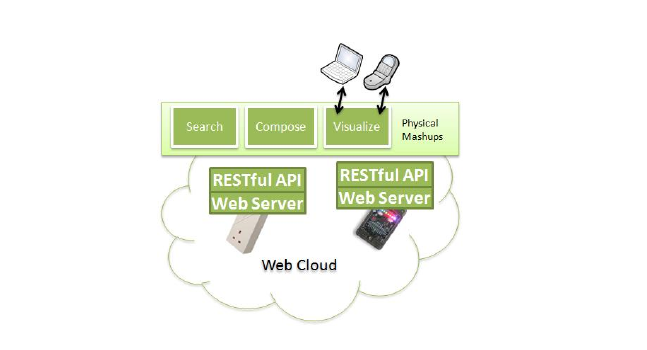
\includegraphics[width=0.9\textwidth]{figuras/figura_2_4}
    \caption{Integração direta dos dispositivos do mundo real através do IP.}
    \label{http-embarcado}
\end{figure}
\begin{figure}[h!]
   \centering
   \subfloat[]{
	   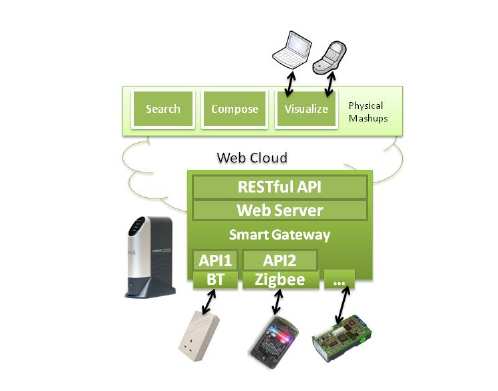
\includegraphics[width=0.5\textwidth]{figuras/figura_2_5_a}
   }
   \subfloat[]{
	   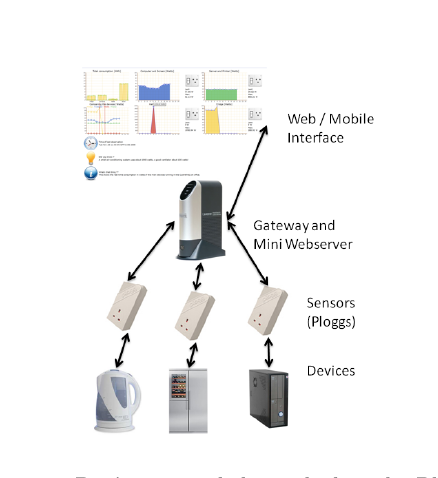
\includegraphics[width=0.5\textwidth]{figuras/figura_2_5_b}
   }\caption{Arquitetura de integração utilizando \emph{Smart Gateway}.}
    \label{http-centralizado}
\end{figure}

%% Falta citar a referencia de onde as figuras foram retiradas

Para este trabalho, foi escolhido o segundo modelo, pois o microcontrolador utilizado no protótipo não possui nenhum \emph{HTTP Server} já implementado ou qualquer biblioteca disponível, portanto, para o primeiro modelo, haveria a necessidade de desenvolver tal estrutura o que não é o propósito deste trabalho.

Por fins didáticos, a estrutura escolhida será dividida em três níveis:
\begin{itemize}
    \item \textbf{Rede de Atuadores e Sensores Sem Fio (RASSF)} - constitui-se dos dispositivos (atuadores e sensores) que interagem com o ambiente e aparelhos de modo a prover serviços. O papel destes dispositivos é coletar dados do ambiente e executar ações apropriadas baseadas nos mesmos e/ou nas requisições das camadas acima (cliente/usuário ou SG). No protótipo deste trabalho tais dispositivos serão desenvolvidos utilizado o microcontrolador Arduino, como dito no início deste capítulo;
    \item \textbf{\emph{Smart Gateway} (SG)} - constitui-se da estrutura responsável por permitir o acesso dos serviços providos pela RASSF através da Web. O seu objetivo central é abstrair os protocolos de comunicação proprietários ou APIs dos dispositivos e prover acesso às suas funcionalidades via RESTful;
    \item \textbf{Aplicação} - constitui-se do componente responsável por emitir um conjunto de consultas ou interesses, que descrevem as características dos fenômenos físicos que o usuário deseja analisar ou requisitar alterações/ações. Como este trabalho prima por acessibilidade, nesta camada foi desenvolvido um sistema de reconhecimento da fala para o português brasileiro no Sistema Operacional Android na versão 3.2 de sua API, formando um estrutura \emph{command-control} acessível aos usuários.
\end{itemize}

%
% Fundamentos referentes à camada de aplicação
%
\section{Android}

\begin{center}
\begin{minipage}{.8\textwidth}
\emph{``The first truly open and comprehensive platform for mobile devices, all the software to run a mobile phone but without the proprietary obstacle that have bindered mobile innovation.''}
\begin{flushright}
    \begin{minipage}{.3\textwidth}
	\emph{Andy Rubin}\cite{Andy Rubin}
    \end{minipage}
\end{flushright}

\end{minipage}
\end{center}

Em dias anteriores ao Twitter e Facebook, quando a Google não passava de um vislumbre nos olhos de seus fundadores, telefones móveis eram apenas isto - aparelhos portáteis tão pequenos que cabiam em pastas e munidos de baterias que podiam durar várias horas. E, além disso, ofereciam a liberdade de fazer ligações sem estarem fisicamente conectados a uma linha.

Incrivelmente pequenos, estilosos e dotados de funcionalidades os telefones móveis hoje são indispensáveis para vida cotidiana. Os avanços em \emph{hardware} os fizeram menores e mais eficientes enquanto eram inclusos inúmeros periféricos. Após as câmeras e os tocadores de música, estes possuem GPS, acelerômetros e telas \emph{touch screens}. E mais, estas inovações em \emph{hardware} forneceram um campo fértil para o desenvolvimento em \emph{software}.

Originário de um grupo de companhias conhecido como \emph{Open Handset Allience - OHA} liderado pela \emph{Google}, o \emph{Android} é uma nova estrutura de sistema operacional desenvolvida para dispositivos móveis com grande poder de \emph{hardware}. Hoje muitas companhias, tanto membros originais da OHA e outras, tem investido intensamente neste sistema, de modo a alocar significativos recursos de engenharia para aperfeiçoar o sistema operacional e trazer dispositivos que o portam ao mercado.

O \emph{Windows Mobile}, o \emph{iPhone} da \emph{Apple} e o \emph{Palm Pre} provêem um  ambiente de desenvolvimento rico e simples para aplicações móveis. Entretanto, diferente do \emph{Android}, estes são construídos em sistemas operacionais proprietários que, em certos casos priorizam aplicações nativas em detrimento das feitas por terceiros, assim como, em certos casos, restringem e/ou controlam a veiculação das mesmas, alem de se limitarem a comunicação entre aplicações e dados nativas.

Em oposição às estruturas supracitadas, o \emph{Android} oferece uma nova possibilidade para aplicações móveis disponibilizando um ambiente de desenvolvimento baseado no \emph{kernel Linux} o qual é \emph{open-source}. O acesso ao \emph{hardware} é permitido a todas aplicações através de uma série de bibliotecas e interações entre as aplicações nativas. Todas as aplicações possuem o mesmo grau de importância, sejam elas nativas ou de terceiros, pois ambos os grupos são desenvolvidos com a mesma API, executadas no mesmo tempo de execução e o usuário pode remover/substituir qualquer aplicação nativa, até mesmo o discador ou a interface do painel principal e substituir por uma sua, se este for o caso.

Desta forma, o Android SDK facilita a integração de entradas de fala em aplicações de terceiros. Para tal, faz-se uso do serviço de reconhecimento em dispositivos, o qual está registrado para receber a \emph{RecognizerIntent}\cite{recintent}. Um grande exemplo é o aplicativo \emph{Google's Voice Search}, que vem instalado na maioria dos dispositivos com sistema operacional Android, este responde a \emph{RecognizerIntent} enviando \emph{streams} de áudio ao servidor da Google onde é processado e retorna um conjunto com os resultados mais prováveis, com base em seus dados. O grande empecilho está no fato de o aparelho necessitar estar conectado à internet. Portanto, sem rede o sistema de reconhecimento não funciona. Entretanto, para o propósito deste trabalho isso é o suficiente.

\section{Sistema para Reconhecimento da Fala}

A implementação de um Sistema de Reconhecimento de Fala pode ser dividida basicamente em duas etapas: treinamento e teste. Previamente à etapa de treinamento é realizada a extração de parâmetros do sinal, ou seja, o áudio presente na base é transformado em coeficientes que servirão de entrada para a etapa de treinamento.

Na etapa de treinamento são realizados o treinamento do modelo acústico e do modelo de linguagem. O primeiro tem como propósito calcular a verossimilhança de uma sequência de vetores acústicos dado um modelo, enquanto o segundo tem por objetivo mapear os relacionamentos entre palavras, estimando a probabilidade de ocorrência de uma palavra em função das anteriores.

A fase de testes compreende o reconhecimento em si, também conhecido como decodificação. Esta fase representa não apenas um problema de reconhecimento de padrões como um problema de busca em um grafo, tendo por objetivo buscar a sequência de palavras que melhor se adapta aos vetores acústicos de entrada, dados os modelos. Então, realiza-se a análise dos resultados, retirando-se então as medidas de interesse. O diagrama apresentado na Figura \ref{fig:CSR} ilustra, de forma resumida, as etapas mencionadas.

\begin{figure}[h!]
\centering
\fbox{
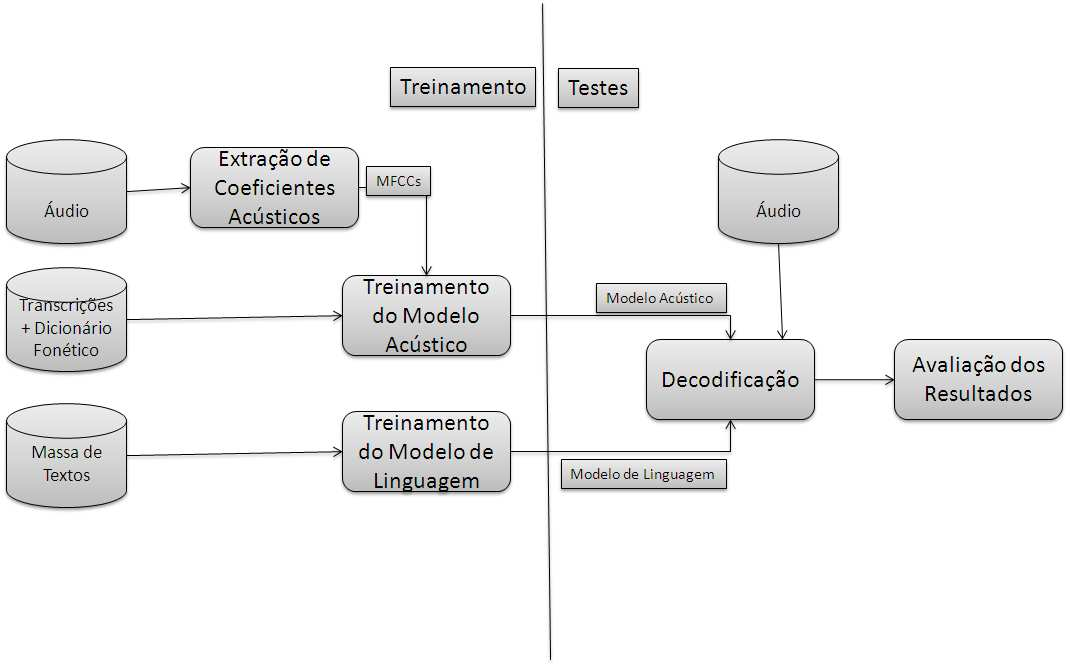
\includegraphics[width=1\textwidth]{figuras/figura_2_1}
p}\caption{Diagrama das etapas envolvidas em um sistema CSR.}
\label{fig:CSR}
\end{figure}

\subsection{Extração de Parâmetros do Sinal}

Para que seja possível processar o sinal de fala para geração do sistema de reconhecimento, torna-se necessária, em uma primeira etapa, a conversão da onda sonora em um sinal digital, que pode ser compreendido pelo computador. O processamento do sinal de fala consiste na amostragem do sinal, janelamento e extração de parâmetros que serão relevantes para o processo de reconhecimento. A extração dos parâmetros é um dos assuntos mais importantes na área de reconhecimento de fala.

A função principal desta etapa de extração de parâmetros é a da divisão do sinal em blocos - supondo que o sinal de fala pode ser considerado estacionário durante um período de tempo muito pequeno, de alguns milissegundos - e derivação de uma estimativa suavizada do espectro a partir de cada bloco. Em um configuração considerada padrão, esses blocos - usualmente chamados de janelas - possuem duração de 25ms e são obtidos a cada 10ms (o que é conhecido por \emph{frame shift}). Ainda, o sistema usa blocos sobrepostos de forma a capturar a informação contida nos seus limites.

Após essa fase, é aplicada uma transformada de Fourier a cada bloco, passando os valores obtidos do domínio do tempo para o domínio da frequência. Depois é feita uma filtragem, com o objetivo de extrair os parâmetros que permitam mais facilmente o reconhecimento da fala. A saída é um vetor de valores filtrados, comumente chamados de mel-spectrum \cite{Cepstrum}, cada um correspondendo ao resultado da filtragem do espectro de frequências da entrada por um filtro individual. Então, o comprimento do vetor de saída é igual ao número de filtros criados. As constantes que definem essa filtragem são o número de filtros (cujas frequências centrais estão em uma escala logarítimica, conforme o ouvido humano), a frequência mínima e a frequência máxima. As frequências máxima e mínima dependem da origem do sinal de voz. Para uma fala em um sistema de telefonia, com frequências de corte de 300 e 3700 Hz, o uso de limites fora desses valores significa apenas perda de banda.

Para uma fala clara, a frequência mínima deve estar acima de 100 Hz, para livrar-se de possíveis interferências da corrente alternada (50/60 Hz) e também porque normalmente não informação útil abaixo desta frequência.

A frequência máxima deve ser menor que a frequência de Nyquist, ou seja, menor que metade da frequência de amostragem. Além disso, acima de 6800 Hz não há muito que possa ser usado para melhorar a separação entre os modelos. Para canais muito ruidosos, uma frequência máxima em torno de 5000 Hz deve ajudar a diminuir o ruído.
Davis e Mermelstein \cite{davis-mermelstein} mostraram que os coeficientes de frequência Mel-cepstrais apresentam características robustas para um bom reconhecimento de fala.

A Figura \ref{fig:extracao} ilustra de forma resumida o processo de extração de parâmetros do sinal.

\begin{figure}[h!]
\centering
\fbox{
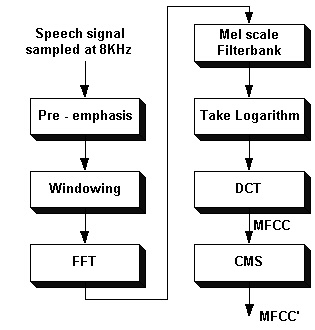
\includegraphics[scale=0.7]{figuras/figura_2_2}
}\caption{Diagrama do processo de extração de parâmetros de um sinal de voz.}
\label{fig:extracao}
\end{figure}

\subsection{Modelagem Acústica}

A modelagem acústica consiste em um método para calcular a verossimilhança de uma sequência de vetores X, dado um modelo M. Os Modelos Ocultos de Markov ou \emph{Hidden Markov Models (HMMs)} são considerados o estado da arte para modelagem acústica.

Os HMMs podem modelar uma unidade menor da palavra (como os fonemas ou mesmo fonemas inseridos em contextos diferentes, como difones ou trifones), uma palavra, ou ainda uma frase inteira.

Os HMMs podem ser vistos como máquinas de estado finitas, onde a cada unidade de tempo ocorre uma transição entre estados e cada estado emite um vetor acústico com uma função densidade de probabilidade associada. Um modelo M pode ser escrito como na Equação \ref{equ:modeloM}.

\begin{equation}
M = A,B,\Pi = a_{ij} , bi, \pi_{i}, i, j = 1, ...,N
\label{equ:modeloM}
\end{equation}

A Figura \ref{fig:exemploHMM} representa um HMM com três estados emissores, onde são adicionados dois estados não emissores no início e no fim do modelo para fins de facilitar a união entre modelos. Na figura, $x_t$ representa um vetor acústico emitido em uma unidade de tempo $t$. Nesta figura, a probabilidade de emissão de um vetor acústico por um estado é representada por uma mistura de gaussianas.

\begin{figure}[h!]
\centering
\fbox{
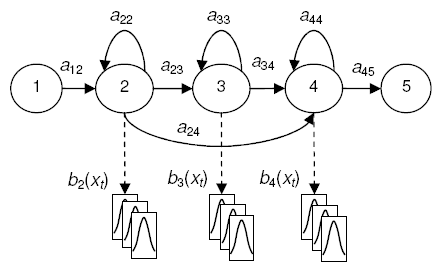
\includegraphics[width=1\textwidth]{figuras/figura_2_3}
}\caption{Exemplo de HMM com três estados emissores}
\label{fig:exemploHMM}
\end{figure}

O objetivo da modelagem é encontrar o ajuste dos parâmetros do modelo que maximize a verossimilhança. Isto é feito através de um algoritmo de reestimação de parâmetros. Dentre eles, o mais usado é o algoritmo de Baum-Welch, também conhecido como \emph{Forward-Backward Algorithm} ou algoritmo de avanço-retorno. Além de todos os parâmetros presentes na mistura de gaussianas associada a cada estado, como médias e variâncias, as matrizes de transição entre estados também são consideradas parâmetros do modelo.

Ainda, de modo a otimizar esses modelos, pode-se utilizar uma técnica de compartilhamento de estados na ocasião do treinamento de fonemas inseridos em contextos diferentes, como no caso dos trifones. Esta técnica pressupõe que alguns fonemas inseridos em diferentes contextos podem não produzir uma variabilidade acústica suficientemente grande para que sejam modelados por HMMs diferentes. Assim, esses trifones podem ser agrupados dentro de um mesmo modelo, através de uma técnica de agrupamento de estados. Geralmente, utilizam-se algoritmos de árvores de decisão.
Através dessa técnica, constrói-se uma árvore para cada fonema, onde o nó pai corresponde a todos os estados com todos os diferentes contextos em que aquele fonema pode ser inserido (no caso de trifones, contexto à direita e contexto à esquerda), ou seja, mesmo fonema central. Os arcos dessa árvore correspondem a perguntas fonéticas que servirão para agrupar estados dentro de categorias diferentes e, por fim, os estados que caírem dentro de um mesmo nó folha serão agrupados como um único estado.

\subsection{Modelo de Linguagem}

O modelo de linguagem provê uma estrutura que define uma inter-relação entre as palavras. De forma geral, estas estruturas são classificadas entre duas categorias: gramáticas de grafos dirigidos ou modelos estocásticos N-Gram. As gramáticas de grafos dirigidos representam um grafo dirigido de palavras onde cada palavra encontra-se em um vértice e cada arco representa a probabilidade de transição entre estas duas palavras (vértices). Já o modelo estocástico gera probabilidades para as palavras baseado na observação das n-1 palavras anteriores (ver \cite{fsr}). Como falado anteriormente, neste trabalho será utilizado um sistema de reconhecimento de palavras isoladas onde o modelo de linguagem é classificado como uma gramática de grafo dirigido onde cada aresta tem peso constante, ou seja, a probabilidade de transição entre palavras é constante para qualquer palavra.

\subsection{Decodificação}

A etapa de decodificação ocorre durante a fase de testes e consiste em uma busca pela sequência de palavras que melhor se adapta aos vetores acústicos, dados os modelos, ou seja, realiza-se uma busca pela sequência de estados que maximiza a chamada probabilidade a posteriori, que pode ser calculada através da fórmula de Bayes, como mostrado na Equação \ref{equ:bayes}.
\begin{equation}
P(W|X) = \frac{P(X|W)P(W)}{P(X)}
\label{equ:bayes}
\end{equation}

Uma vez que, para fins de reconhecimento de fala, o elemento observado não corresponde a um único elemento e sim a uma sequência de vetores acústicos, então, para uma sequência de X vetores, considerando a ocorrência de cada observação como um evento independente, pode-se construir uma regra de decisão $\widehat{W}$ para o problema através da maximização da probabilidade a posteriori, como mostrado na Equação \ref{equ:decisao}. Nesta equação, ainda é possível notar a eliminação do termo presente no denominador da Equação \ref{equ:decisao}. A ausência deste termo é justificável, uma vez que ele será o mesmo para todas as classes testadas.

\begin{align}
\begin{split}
\widehat{W} &= arg \max _{W} P(W|X) \\
&= arg \max _{W} \frac{P(X|W)P(W)}{P(X)} \\
&= arg \max _{W} P(X|W)P(W)
\end{split}
\label{equ:decisao}
\end{align}

É fácil verificar que a chamada probabilidade a priori P(W) da Equação \ref{equ:decisao} será fornecida pelo modelo de linguagem e a probabilidade condicional P(X|W) será fornecida pelo modelo acústico. Logo, onde se lê probabilidade a priori, leremos a probabilidade de ocorrer uma determinada sequência de palavras e onde se lê probabilidade condicional, leremos a probabilidade de observar uma determinada sequência de vetores dada uma sequência de palavras.

O algoritmo mais utilizado nesta etapa de decodificação é conhecido como algoritmo de Viterbi. Ele consiste em um algoritmo de busca síncrono, que procura pelo estado mais provável a cada unidade de tempo. Este algoritmo considera uma aproximação, conhecida por aproximação de Viterbi. Como mostrado na Equação \ref{equ:viterbi}, esta aproximação considera que, como o objetivo da decodificação é encontrar a melhor sequência de palavras, então, o somatório da
Equação \ref{equ:decisao} pode ser substituído pelo máximo, de forma a encontrar a melhor sequência de estados.

\begin{equation}
\widehat{W} = arg \max _{W} P(W|X) \cong arg \max _{W} [P(W) \max _{s_{0}^{T}} P(X,s_{0}^{T}|W)]
\label{equ:viterbi}
\end{equation}

De forma a melhorar o desempenho da busca, o decodificador usa duas estratégias: guardar alguns caminhos ótimos intermediários, de forma que alguns resultados possam ser usados por outros caminhos sem que haja necessidade de computá-los novamente, além de realizar poda nos nós que se encontram abaixo de um limiar pré-estabelecido. Desta forma, a cada passo, o decodificador elimina caminhos que são muito provavelmente desnecessários, percorrendo apenas um feixe do espaço de busca. Este tipo de busca é conhecido como busca em feixe.

\section{Arduino}

\begin{figure}[h!]
\centering
\fbox{
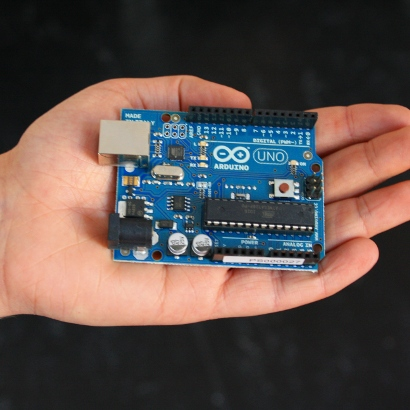
\includegraphics[width=0.5\textwidth]{figuras/arduino_uno}
}\caption{Arduino UNO utilizado neste trabalho.}
\label{fig:arduino}
\end{figure}

Arduino \cite{arduino} é uma plataforma de prototipagem eletrônica \emph{opem-source} baseada em flexibilidade, fácil acesso ao \emph{hardware} e \emph{software} destinada a artistas, \emph{designers}, curiosos ou qualquer pessoa interessada em criar objetos ou ambientes interativos.

Originalmente, este microcontrolador, foi criado como uma plataforma educacional para uma classe de projetos da \emph{Interaction Desing Institute Ivrea} em 2005 com o intuito de suportar mentes artísticas e baseadas a \emph{design}. Focado em simplicidade, busca uma estrutura voltada para um público sem muita base tecnológica.

O Arduino pode perceber o ambiente através de entradas oriundas de uma variedade de sensores e é capaz de executar ações ao seu redor usando controles de luz, motores e outros atuadores. Seu microcontrolador é programado usando a linguagem de programação Arduino \cite{arduinoapi} (baseado em \emph{Wiring} \cite{wiring}) e o ambiente de desenvolvimento Arduino (desenvolvido em Java e baseado em \emph{Processing} \cite{processing}). Projetos em Arduino podem ser auto-suficientes (quando executam sem interferências externas) ou comunicando-se com \emph{softwares} em um computador usando um cabo USB ou combinado com algum componente que permita tráfego de dados sem fio (Ex.: \emph{Shield Bluetooth}).

Oferecendo tudo que é necessário para uma comunicação ubíqua \cite{Mark Weiser}, sua utilização cresceu de tal maneira que ultrapassou o domínio para o qual foi inicialmente proposto. Hoje é usado nas mais diferentes gamas onde este trabalho é um grande exemplo, pois, sua facilidade de manuseio e a flexibilidade em agregar componentes otimizando a integração com outros dispositivos o torna candidato ideal, posto que, como dito inicialmente, a integração é o ponto chave na implementação de uma \emph{Web of Things}.

\chapter{Funcionamento do Sistema}
\label{chap:funcionamento}

Neste capítulo será apresentado o protótipo do sistema proposto no início deste documento. Para tal, como foi feito no Capitulo 2, o sistema será dividido em níveis:

\begin{itemize}
    \item \textbf{RASSF} - será apresentada na primeira seção, de modo a explicitar quais componentes físicos foram utilizados e a arquitetura do programa interno;
    \item \textbf{SG} - será apresentado na segunda seção, e como o item anterior, explicita quais componentes físicos foram utilizados e a arquitetura do programa interno, além de introduzir uma abordagem relativamente diferente da apresentada no trabalho referenciado por \cite{sgtriwiguiboh}, dadas as diferenças de Linguagens de Programação utilizadas na base do sistema;
    \item \textbf{Aplicação} -  será apresentada na terceira seção, expondo como o sistema de reconhecimento de fala para Android foi desenvolvido, assim como todo o processo de preparação dos dados, extração de coeficientes e treinamento dos modelos acústico e linguístico. Também será vista a arquitetura implementada para o Cliente REST.
\end{itemize}

\section{Rede de Atuadores e Sensores Sem Fio (RASSF)}

Na RASSF, os papéis dos sensores e atuadores é coletar dados do ambiente e executar apropriadas ações baseadas nos mesmos e/ou nas requisições das camadas a cima.

Os sensores detectam os fenômenos do ambiente e transmitem esses dados para os atuadores para que eles executem as devidas ações. Entretanto, estes podem ser enviados para o SG, o qual pode delegar aos atuadores a execução das ações cabíveis. Esta estrutura de ação é chamada Arquitetura Autônoma (Figura \ref{fig:arquitetura-autonoma} (a)), pois não há existência de intervenção humana. Quando o dado, ao invés de ser processado e executado na própria rede, é enviado para a camada de aplicação através do SG solicitando uma intervenção humana, a estrutura é chamada de Arquitetura Semi-Autônoma (Figura \ref{fig:arquitetura-autonoma} (b)), desde que a ação seja coordenada pelo SG.

\begin{figure}[htbp]
   \centering
    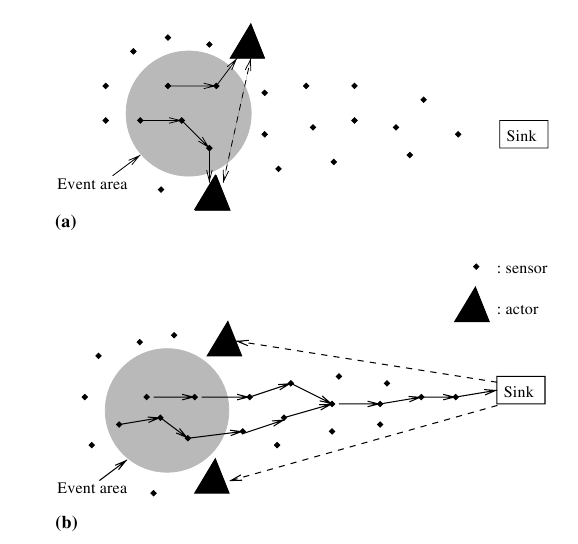
\includegraphics[width=0.6\textwidth]{figuras/figura_2_6}
    \caption{Arquitetura (a) Autônoma e (b) Semi-Autônoma.}
    \label{fig:arquitetura-autonoma}
\end{figure}

Dependendo da funcionalidade a ser agregada, uma das duas arquiteturas deve ser usada, ou até mesmo as duas. Como esta sendo proposto um sistema \emph{command-control}, a arquitetura semi-autônoma é a mais propícia, entretanto, para acessibilidade, quanto mais autônoma a arquitetura for, mediante configurações iniciais, maior a independência do usuário. De modo a resolver este dilema o sistema foi implementado utilizando a arquitetura semi-autônoma como base, mas com flexibilidade suficiente para expandi-la e/ou combiná-la com uma arquitetura autônoma dependendo da demanda.

Os componentes dos nós sensores e atuadores de uma RASSF podem ser vistos na Figura \ref{fig:componentes-atuador-sensor} (a) e (b), respectivamente.

\begin{figure}[htbp]
   \centering
    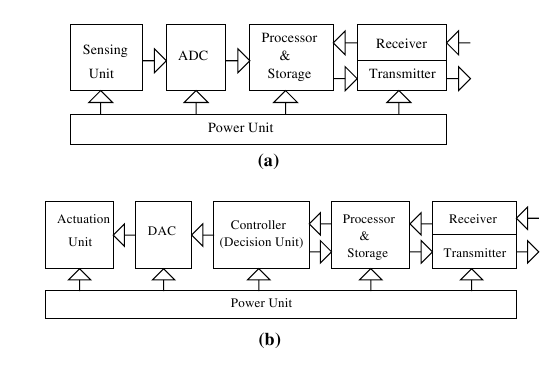
\includegraphics[width=0.6\textwidth]{figuras/figura_2_7}
    \caption{Componentes dos (a) sensores e (b) atuadores.}
    \label{fig:componentes-atuador-sensor}
\end{figure}

Os nós sensores são equipamentos possuidores de uma unidade de força, subsistemas de comunicação (transmissor e receptor), recursos de armazenagem e processamento, Conversores Analógicos para Digitais (\emph{Analog to Digital Converter - ADC}) e unidade de sensoriamento. A unidade de Sensoriamento possui a tarefa de observar fenômenos como: eventos térmicos, óticos ou acústicos. O dado é coletado de forma analógica e convertido para digital através do ADC, daí é analisado pelo processador e então transmitido para os atuadores cabíveis.

A função da unidade de decisão (controlador) é receber a leitura do sensor como entrada e gerar um comando de ação como saída. Tais comandos são convertidos em dados analógicos por um Conversor Digital para Analógico (\emph{Digital to Analog Converter - DAC}) e são transformados em ações pelas unidades de atuação.

Todas as necessidades citadas anteriormente são supridas pelo Arduino UNO, o que combinado com sua facilidade e flexibilidade de desenvolvimento, o tornaram candidato ideal para ser escolhido de modo a compor a rede de atuação e sensoriamento.

Além disso, uma RASSF possui duas características básicas \cite{wsaniais}:
\begin{itemize}
    \item \textbf{Requerimentos em tempo real}: Em RASSF, dependendo da situação, há a necessidade de uma rápida resposta para em determinado evento. Por exemplo, em incêndio, as ações devem ser iniciadas na área do evento o quanto antes. Além disso os dados coletados devem continuar válidos até o momento da ação.
    \item \textbf{Coordenação} - Diferentemente das redes de sensores onde a entidade central é responsável pela coleta e processamento dos dados, em  uma RASSF ocorre um outro fenômenos chamado sensores-atuadores e atuadores-atuadores, os quais pode ser vistos no trabalho referenciado por \cite{wsaniais}.
\end{itemize}

Neste trabalho a característica coordenação supracitada não foi implementada, pois foi utilizado apenas um componente atuador que possui a função de controlar um televisor através de um emissor \emph{Infra Red}. Desta forma, somente a característica de requerimento em tempo real se fez necessária, pois, apesar de não ser utilizada neste protótipo, objetivou-se a possível expansão do sistema para uma arquitetura autônoma, como dito anteriormente.

A implementação do programa residente no Arduino capaz de executar as ações requeridas pelo usuário, i.e., controlar efetivamente o aparelho televisor através de um emissor \emph{Infravermelho}, foi facilitada devido à utilização da biblioteca IRRemote. Entretanto, para seu perfeito funcionamento, há a necessidade do trenamento da base, o qual consiste na obtenção dos códigos do controle remoto referente à televisão que se deseja controlar. Este treinamento é feito com a própria biblioteca que possui a capacidade de decodificar o sinal de entrada, com o auxílio de um leitor \emph{Infravermelho}. Infelizmente, no período de desenvolvimento deste trabalho, este material, leitor \emph{Infravermelho}, não estava disponível. Portanto, afim de encontrar uma maneira alternativa de provar o conceito proposto sem perder generalidade ou fugir do escopo, o emissor foi substituído por um LED, pois este, apesar de não ser capaz de controlar um televisor, emula a execução do comando de maneira visível e de fácil percepção.

\section{Smart Gateway (SG)}
\label{sec:sg}

Hoje, como a integração direta de dispositivos com a Web ainda é extremamente difícil, dado que muitos destes não suportam protocolos para esses fins, como \emph{Internet Protocol (IP)} ou HTTP que são comumente utilizados em RASSF, uma abordagem diferenciada se faz necessário. O trabalho \cite{wotdovad} propõe o uso do conceito SG como elemento intermediário, propiciando o acesso aos dispositivos pela Web. O objetivo central do SG é abstrair os protocolos de comunicação proprietários ou APIs dos dispositivos e prover acesso às suas funcionalidades via RESTful.

Segundo o trabalho referenciado por \cite{sgtriwiguiboh}, a arquitetura de um SG deve ser projetada com base em três princípios: simplicidade, extensibilidade e modularidade. Simplicidade e extensibilidade para permitir a extensão e a customização para atender as necessidades dos usuários. E, modularidade, para que os componentes internos possam interagir através de pequenas interfaces, permitindo assim, a evolução e troca das partes individuais do sistema.

Para tal, sua arquitetura deve ser composta por três camadas principais: camada de apresentação, camada de controle e camada de abstração. A Figura \ref{fig:estrutura-sg} mostra, de forma geral, esta estrutura.

\begin{figure}[htbp]
   \centering
    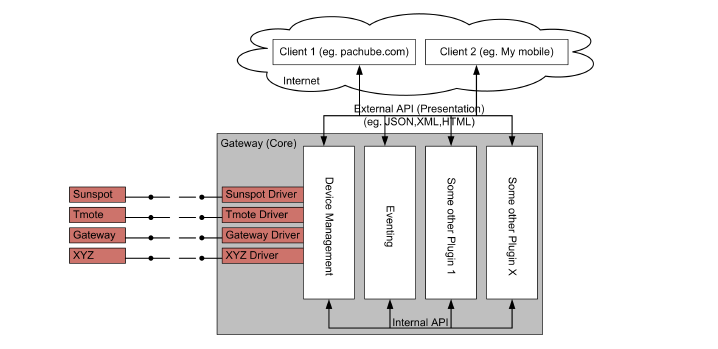
\includegraphics[width=1\textwidth]{figuras/figura_2_8}
    \caption{Visualização em alto nível de um \emph{Smart Gateway}.}
    \label{fig:estrutura-sg}
\end{figure}

Diferente da linguagem utilizada no último trabalho referenciado, uma abordagem diferente foi tomada, pois a linguagem Python oferece uma unidade organizacional que tem por base os três princípios de um SG. Esta arquitetura é chamada de módulo.

Mark Lutz \cite{python} define módulo como a unidade organizacional de programação de alto nível que empacota códigos de programas e dados para reuso. Em termos concretos, módulos geralmente correspondem a arquivos de programas em Python ou extensões de código em linguagens externas como C, Java, C\# ou etc, onde cada arquivo é um módulo e um módulo importa outros módulos para usar os nomes definidos por estes. Desta forma, os módulos provêem um modo mais fácil de organizar componentes em um sistema. O que é objetivado por um SG.

A seguir será apresentado o funcionamento de cada estrutura do SG (Figura \ref{fig:estrutura-sg}) e como foi adaptada para o Python quando isto se fez necessário.

\subsection{Camada de Apresentação}

A camada de Apresentação torna os componentes do SG acessíveis para a Web. Sendo uma fina camada acima da camada de controle, que gerencia as requisições dos clientes através de uma interface REST.

Com o intuito de tornar os dispositivos acessíveis através da Web, um mapeamento dos nomes dos dispositivos em \emph{Uniform Resource Identifier (URI)} \cite{w3curi} é executado pela camada de apresentação. O dispositivo nomeado ``sensor1'' será mapeado por ``/sensor1''. Isto permite aos usuários procurar dinamicamente a lista de dispositivos.

Requisições da Web utilizando este mapeamento serão redirecionadas para o \emph{driver} referente ao dispositivo informado, o qual, tratará a solicitação e gerará uma resposta.

Na implementação desta camada nenhuma adaptação foi exigida. A biblioteca/módulo BaseHTTPServer supriu as necessidades do servidor HTTP gerando apenas a obrigatoriedade da definição do mapeamento anteriormente citado.

\subsection{Camada de Controle}

A camada de controle é composta por diversos componentes independentes chamados plugins.

Um plugin é um componente de software que é carregado na fase de iniciação do SG . Sua principal funcionalidade é permitir a acoplagem eficiente dos drivers e, assim, possibilitar o direcionamento, sem ambiguidade, das requisições da camada acima (Camada de Apresentação) para os seus respectivos drivers.

É permitido a um plugin depender de outros. Entretanto, para manter uma fraca dependência entre os mesmos, deve ser utilizado um mecanismo de sincronização de modo que, ao ocorrer uma mudança no estado de qualquer dispositivo, o sistema consiga percebê-la e reorganizar-se ao ponto de não permitir as requisições quando não houver recurso disponível (exemplo: o plugin de um determinado dispositivo chama seu método independente do dispositivo estar ausente ou não).

Como este trabalho consiste de um sistema extremamente simples existindo apenas um único driver, como será explicitado a seguir, a única funcionalidade desenvolvida nesta camada consiste no mecanismo de sincronização acima definido, de modo a impedir as requisições inexistentes por falta de recursos.

\subsection{Camada de Abstração}

Como na maioria dos sistemas operacionais modernos, o SG provê uma camada de abstração para os dispositivos. Para as aplicações no nível acima, todos os dispositivos são vistos da mesma forma, mesmos aqueles com implementações completamente diferentes.

A camada de abstração é ilustrada ao lado esquerdo da Figura \ref{fig:estrutura-sg}. Drivers especializados são usados para se comunicar através de seus protocolos proprietários com os respectivos dispositivos físicos (SunSpotDriver utiliza ZigBee com SunSpot).

Para dispositivos que já suportam protocolos Web, a implementação do \emph{driver} trabalha apenas repassando as requisições da camada de apresentação para os dispositivos. Entretanto, quando o dispositivo não suporta protocolos Web, o \emph{driver} é responsável por traduzir a requisição para seu protocolo de modo a fazer o dispositivo compreendê-lo.

Como não foi encontrado no período de desenvolvimento deste trabalho um componente para o Arduino que o permitisse suportar protocolos Web, o uso de qualquer protocolo de comunicação entre ele e o SG não trouxe grande variação, pois, para qualquer padrão utilizado haveria a necessidade da implementação de um \emph{driver} nesta camada. Logo, sem perdas de generalidade, o protocolo escolhido foi o 802.15 \emph{Bluetooth}. O que consequentemente demandou o desenvolvimento do seu respectivo \emph{driver} que foi facilitado graças à utilização da biblioteca/módulo Bleuz.

\section{Aplicação}
\label{sec:aplicacao}

A aplicação é o componente responsável por emitir um conjunto de consultas ou interesses, que descrevem as características dos fenômenos físicos que o usuário deseja analisar. Os interesses da aplicação podem indicar os tipos de dados desejados; a frequência com que esses dados devem ser coletados; a necessidade ou não dos dados sofrerem algum tipo de agregação; os limiares a partir dos quais os dados devem ser transmitidos; ou ainda, eventos que podem disparar algum comportamento peculiar da rede, como a ativação de sensores específicos, a alteração na taxa de sensoriamento ou o início de uma ação para os atuadores. Em particular, este último é o de maior relevância, posto que o protótipo proposto consiste de um sistema  \emph{command-control} através da RESTful API.

De modo geral, a ideia central da arquitetura REST reside no conceito de recurso como algum componente de uma aplicação que é valorada por uma identificação única. Na Web as identificações dos recursos é feita pela URI, como dito anteriormente, desta forma os clientes de serviços REST podem seguir esta estrutura para encontrar recursos de modo a interagir com os mesmos, como em navegadores Web. Isto permite aos clientes explorar serviço simplesmente navegando e, em muitos casos, estes vão usar uma variedade de tipos de links para estabelecer diferentes relações entre os recursos disponíveis, estas relações são chamadas de \emph{meshup}. Entretanto, neste trabalho, a geração de tais links não se fez necessário, pois o sistema é extremamente simples e com finalidade de prova de conceito.

Como o SG seguiu a arquitetura REST, é possível acessar os recursos através de qualquer cliente REST, como por exemplo um navegador WEB, desde que se conheça o endereço IP do servidor. Tendo isto em mente, desenvolveu-se uma aplicação para Android com versão 3.2 afim de acessar os recursos disponíveis pelo sistema. Entretanto, apesar da simplicidade da arquitetura do Android, são necessárias algumas considerações para fazer o melhor uso deste sistema.

\subsection{Cliente REST para Android}

Para potencializar sua utilização em um dispositivo cujo seu sistema operacional é Android, a arquitetura montada seguiu os padrões apresentados na Googlo I/O 2010 \cite{restclient}, a qual pode ser vista na Figura \ref{fig:rest_android}.

\begin{figure}[h!]
   \centering
    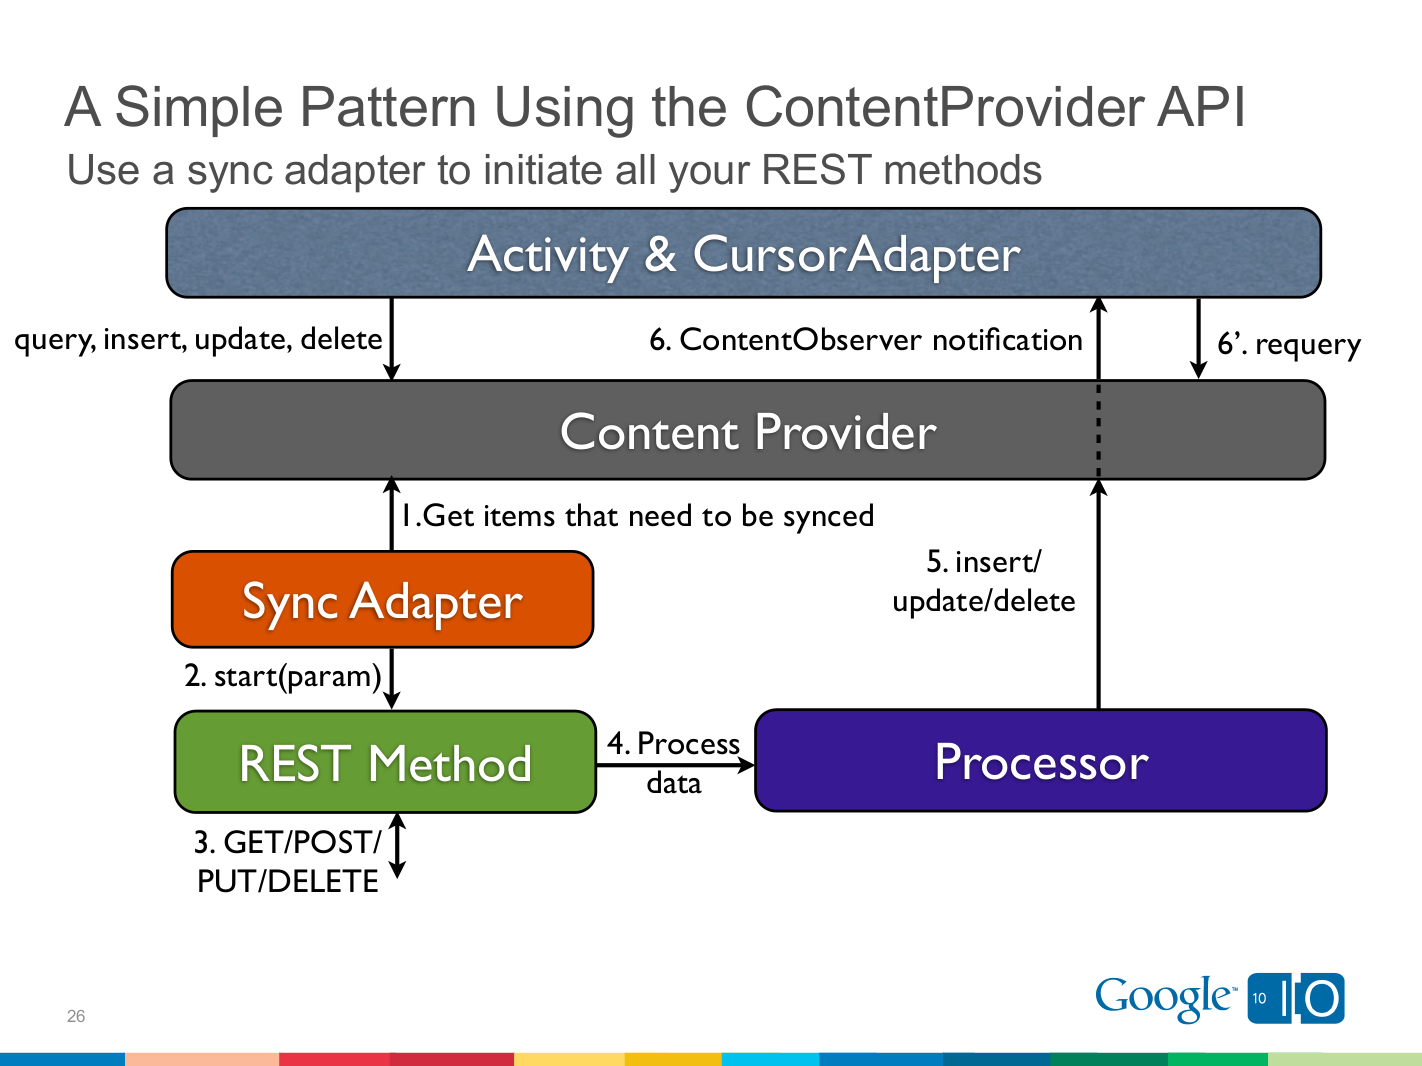
\includegraphics[width=0.8\textwidth]{figuras/rest_android}
    \caption{Arquitetura REST sugerida pela Google 10.}
    \label{fig:rest_android}
\end{figure}

Cada entidade terá suas funções apresentadas brevemente:
\begin{itemize}
    \item \textbf{Método REST} - Concentra a arquitetura do cliente REST
	\begin{itemize}
	    \item Prepara o HTTP URL e o corpo da requisição HTTP;
	    \item Executa a transação HTTP;
	    \item Processa a resposta HTTP;
	    \item Seleciona o tipo de conteúdo opcional para resposta (XML, JSON, Binary);
	    \item Habilita o codificador de conteúdo gzip quando possível;
	    \item Roda o método REST em uma \emph{thread} separada;
	    \item Usa o cliente Apache HTTP.
	\end{itemize}
    \item \textbf{\emph{Sync Adapter}} - Utilizado para executar as operações em \emph{background} de maneira assíncrona;
    \item \textbf{\emph{Processor}} - Concentra a lógica do sistema.
    \item \textbf{\emph{Content Provider}} - Atua como interface entre a \emph{Activity} e o \emph{Processor}/\emph{Sync Adapter} provendo dados e permitindo que a \emph{Activity} possa operar sem interrupção.
    \item \textbf{\emph{Activity \& CursorAdapter}} - Uma \emph{Activity} é o componente da aplicação que prove uma tela com a qual o usuário possa interagir de modo a fazer algo como, discar e efetuar uma ligação, digitar o conteúdo de uma mensagem e enviá-lo, ver um mapa e etc. Já o \emph{CursorAdapter} é um adaptador para expor dados oriundos de uma base.
    \begin{enumerate}
	\item Adiciona a operação de ouvir em \emph{onResume} e removê-lo em \emph{onPause}
	\item Trata as notificações do \emph{ContentProvider}
    \end{enumerate}

\end{itemize}

Neste trabalho o componente \emph{Content Provider} supracitado não foi necessário, pois do REST o método GET foi o único implementado, consequentemente, não gerando transição de dados de um banco.

Apesar da aplicação funcionar de maneira satisfatória, permitindo o acesso aos recursos do SG, esta não garante acessibilidade. Para suprir tal necessidade um novo componente foi desenvolvido. Um sistema \emph{command-control} que utiliza a Google Voice API para reconhecimento da fala, como será mostrado a seguir.

\subsection{Sistema de Reconhecimento de Fala no Android}

Esta tecnologia está disponível desde 2009 com a versão 1.5 de sua plataforma. Inicialmente o servidor da Google suportava Inglês, Mandarim e Japonês. Hoje se estende a diversos idiomas inclusive o Português Brasileiro, o qual será utilizado neste trabalho.

Em versões anteriores ao Android 2.2, não era possível desenvolver qualquer aplicativo utilizando este recurso sem iniciar sua \emph{Activity} quando ativado, sobrepondo a principal. Um exemplo desta estrutura pode ser visto no aplicativo \emph{Handcent SMS} \cite{handcent}, mostrado na figura \ref{fig:handcent-sms}, o qual utiliza esta tecnologia para escrever uma mensagem SMS (versão 1.5 do Android). A partir da versão 2.2, foi desenvolvida uma classe que permite a requisição ao servidor em \emph{background} e mais, esta possui um conjunto de métodos que geram maior controle sobre este serviço e possibilita uma extração mais refinada dos resultados.

\begin{figure}[h!]
   \centering
   \subfloat[]{
	   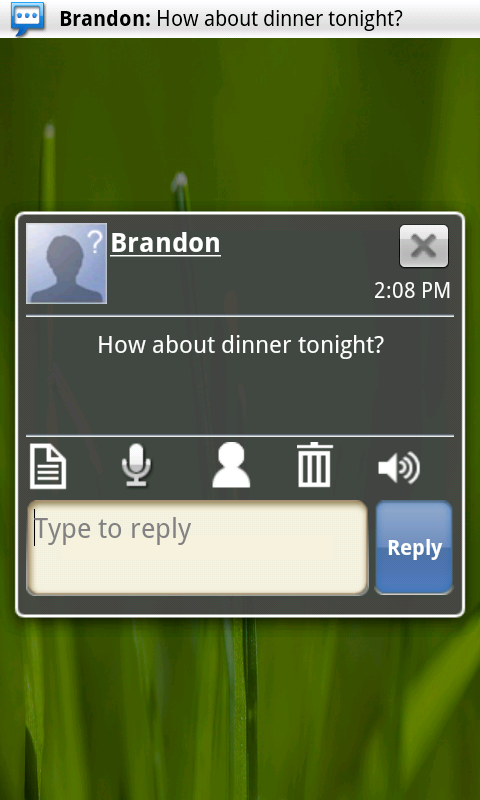
\includegraphics[width=0.3\textwidth]{figuras/GV_sms1}
   }
   \subfloat[]{
	   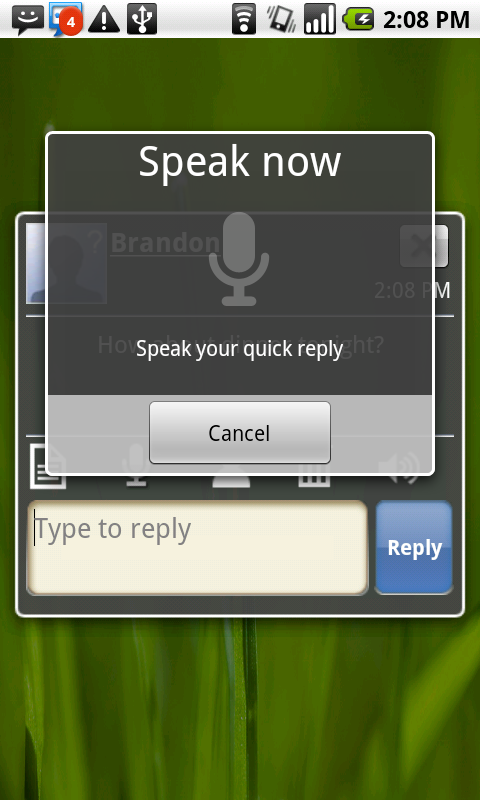
\includegraphics[width=0.3\textwidth]{figuras/GV_sms2}
   }
   \subfloat[]{
	   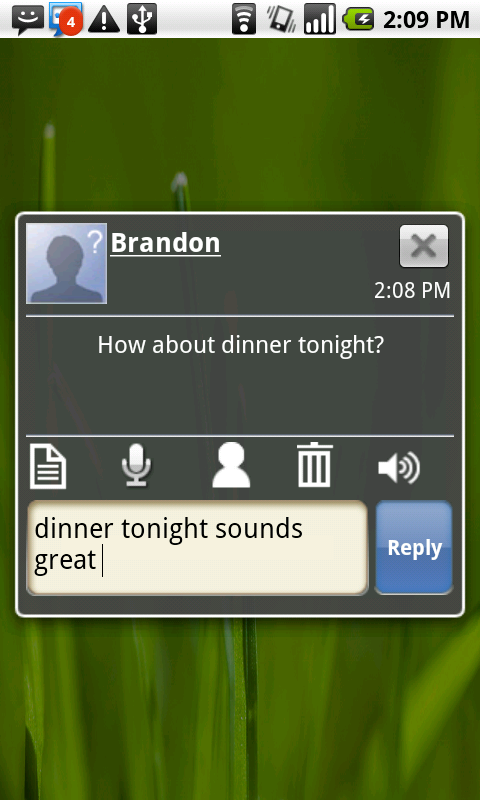
\includegraphics[width=0.3\textwidth]{figuras/GV_sms3}
	   }\caption{Handcent SMS - 05/03/2010 \cite{handcent}}
    \label{fig:handcent-sms}
\end{figure}

Neste protótipo, apesar das requisições ao servidor da Google serem executadas assincronamente em relação ao programa principal e, como a  plataforma utilizada está na versão 3.2, a interface foi moldada de modo a expor alguns dados do reconhecimento (ver figura \ref{fig:tv-control}). Um desses dados é o conjunto dos melhores resultados encontrados pelo servidor da Google, pois este não retorna apenas um comando, o melhor ranqueado, mas sim um conjunto com as melhores estruturas reconhecidas \footnote{É passado uma \emph{stream} de áudio que pode conter uma ou mais palavras}. Logo que esta lista é recebida, é conferido se o comando encontra-se dentre elas e, caso a resposta seja positiva este é dado como reconhecido. É importante ressaltar que para este trabalho foi escolhido o número de quatro melhores resultados de forma a caber na lista de exibição na interface do sistema a qual se localiza no canto esquerdo com um formato de lista ordenada com maior prioridade aquele que foi o melhor ranqueado.

Outro ponto extremamente relevante é conseguido através de algumas manipulações utilizando os recursos da API. Esta possui um conjunto de métodos capazes de saber quando ocorre o início e fim da fala - microfone capta algo diferente de ruido e/ou silêncio e vice-versa - e quando a requisição é enviada ao servidor e os dados são recebidos. Logo, com este conjunto de dados, é possível calcular a relação entre o tempo de processamento do servidor e o tempo do discurso, sem desprezar o tempo de transferência de dados entre o aparelho e o servidor da Google. Este resultado é exposto na base da interface, abaixo do campo expositor do melhor resultado retornado.

A possibilidade destas aferições e a praticidade no manuseio, foram determinantes na escolha da utilização deste recurso em detrimento do desenvolvimento de um sistema de reconhecimento de fala. Posto que a realização deste último foge do objetivo deste trabalho.

Como o SG está instalado em um computador móvel, seu endereço IP não é estático. Desta forma, foi criado um campo de entrada de texto, localizado no topo da interface, para a inserção do respectivo endereço do servidor. E, para haver coesão deste novo campo com o restante do sistema, só é possível fazer qualquer tipo de requisição após a definição deste valor.

\begin{figure}[htbp]
   \centering
    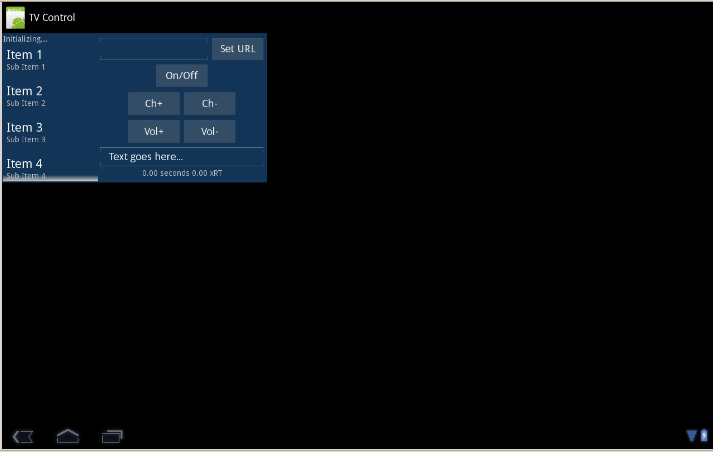
\includegraphics[width=1\textwidth]{figuras/tv_control}
    \caption{TV Control}
    \label{fig:tv-control}
\end{figure}

Visando simplicidade no protótipo, foram definidos 6 comandos representativos do controle remoto. São eles:
\begin{itemize}
    \item Ligar Televisão;
    \item Desligar Televisão;
    \item Subir Canal;
    \item Abaixar Canal;
    \item Subir Volume;
    \item Abaixar Volume.
\end{itemize}

Desta forma foi possível manejar as funções básicas oferecidas pelo aparelho televisor sem perdas de generalidade.

\chapter{Trabalhos Correlatos}
\label{chap:trabalhos-correlatos}

Nos dias atuais muito se fala sobre acessibilidade, entretanto, poucos sabem o que de fato este termo significa. De maneira objetiva, acessibilidade significa não apenas permitir que pessoas com deficiências ou mobilidade reduzida participem de atividades que incluem o uso de produtos, serviços e informação, mas a inclusão e extensão do uso destes por todas as parcelas presentes em uma determinada população.

Para que a acessibilidade atinja níveis funcionais a PCDs com lesões severas, torna-se indispensável a utilização de aparatos eletrotécnicos. Um exemplo muito claro é o Motrix \cite{motrix}. Este programa permite que pessoas com deficiências motoras graves, em especial tetraplegia e distrofia muscular, possam ter acesso aos microcomputadores, permitindo assim, em especial com a intermediação da Internet, um acesso amplo a escrita, leitura e comunicação utilizando apenas a voz.

O uso do Motrix torna viável a execução pelo PCD de quase todas as operações que são realizadas por PSD (Pessoa Sem Deficiência), mesmo as que possuem acionamento físico complexo, tais como jogos. Através de um mecanismo inteligente, o computador realiza a parte motora mais difícil destas tarefas possibilitando assim as ações desejadas.

O Projeto Motrix vem sendo desenvolvido no Núcleo de Computação Eletrônica da Universidade Federal do Rio de Janeiro (UFRJ) desde março/2002 sob coordenação do Professor José Antônio Borges.

Este programa foi a grande inspiração para o sistema desenvolvido neste trabalho. Posto que o objetivo central consiste em expandir as funcionalidades de controle do mundo virtual ao mundo físico, ao ponto do PCD controlar objetos eletrônicos sem o auxílio de PSDs.

Entretanto, controlar objetos físicos ao invés de virtuais é relativamente mais complexo e requer uma abordagem diferenciada. O trabalho \emph{Towards Web of Things} \cite{wotdovad} mostra como tornar objetos do mundo físico acessíveis no mundo virtal. E mais, transforma-os em parte integrante da Web fazendo uso de protocolos abertos. Desta forma, qualquer aplicação que conheça estes padrões pode acessá-los.

O trabalho apresenta dois modos diferentes de integrar os dispositivos via REST:
\begin{itemize}
	\item Integração direta baseado nos avanços da computação embarcada;
	\item A utilização de SGs para dispositivos com recursos limitados.
\end{itemize}

Ambas metodologias foram ilustradas implementando-as em duas plataformas diferentes. Foi mostrado como um eco-sistema de dispositivos RESTful pode facilitar significativamente a criação de \emph{mashups} físico-virtuáis. E neste processo foi constatada a grande flexibilidade e poderoso mecanismo de prototipagem de aplicações que é oferecido pela combinação do REST e a Web para conectar dispositivos.


\chapter{Conclusão}
\label{chap:conclusao}

Este projeto foi extenso e complexo. A sua multi e interdisciplinaridade gera desdobramentos e empecilhos que desafiam o desenvolvedor a ampliar seus horizontes e mudar seu ponto de vista sobre este prisma de integração muitas vezes escondidos de olhos não treinados. Sua complexidade técnica demanda tempo, paciência e dedicação afim de adquirir o mínimo de conhecimento necessário para executar tal tarefa. Entretanto, este cumpre ao que se propõe. Consegue de fato gerar uma certa independência funcional ao grupo objetivado apesar das limitações do usuário, mas não da maneira mais eficiente. É possível fazer diversas alterações e melhorias, como será visto mais adiante.

O sistema de reconhecimento de voz foi testado por uma única pessoa de modo que cada comando foi repetido 20 vezes. Todos os comandos obtiveram um acerto de 100\%, lembrando que as condições foram propícias para tal, ambiente com ruído reduzido, microfone próximo ao orador e fala calma e pausada. Lembrando que este deve estar entre os cinco melhores resultado retornados pelo servidor do Google, como apresentado na Seção \ref{sec:aplicacao}.

A decisão de utilizar plataformas e padrões abertos facilitou a integração dos três módulos desenvolvidos permitindo que estes pudessem se comunicar perfeitamente apesar de suas diferenças em tecnologias. Entretanto, estas diferenças combinadas com suas funcionalidades disjuntas geram uma grande dificuldade. A primeira demanda de tempo para agregar o conhecimento necessário e prática para poder usá-lo adequadamente de modo a gerar a segunda o que, consequentemente, fez com que o desenvolvimento deste protótipo se estendesse por dois anos.

Apesar disso, a implementação do SG mostrou-se mais fácil dentre os três módulos, pois este residi em um notebook dotado de grande poder computacional em comparação com os recursos usados nos demais (Aplicação - \emph{SmartPhone} e RASSF - Arduino). Desta forma foi possível adaptar o módulo à necessidade do sistema sem exigir muitas manobras no desenvolvimento ou agregação de componentes físicos devido sua incapacidade de exercer seu papel.

Por outro lado, a realização da RASSF ou, nesta implementação, o atuador, mostrou-se o mais complexo. Apesar do Arduino ser um componente de fácil utilização e haver muita documentação oficial e não oficial disponível, a avaliação da condição dos componentes físicos e integração do mesmos é muito clara na teoria, mas na prática é obscura e imprecisa. Componentes sem defeitos aparentes funcionam de forma anômala gerando dados incoerentes o que, por consequência, retarda o avanço do projeto. Para contornar esta situação é imprescindível possuir mais de uma réplica do mesmo componente e, até mesmo, mais de uma solução para um mesmo problema. Estas lições foram aprendidas a duras penas e várias horas de tentativas e erros, provando a necessidade da experiência na prototipagem para alcançar o resultado objetivado.

A seguir serão apresentados alguns problemas presentes neste protótipo e possíveis sugestões de melhoras visando trabalhos futuros.

\section{Trabalhos Futuros}

O reconhecimento da fala é algo que aos poucos tem estado cada vez mais presente no dia a dia das pessoas. Telefones celulares, televisores e outros aparelhos estão sedo comercializados com este tipo de sistema integrados desdas fábricas. Contudo, possui problemas que ainda são extremamente desafiadores perante o atual avanço tecnológico e científico. O reconhecimento robusto, que consiste no reconhecimento da fala em ambientes com barulho, pode não possuir um grau de acerto em níveis aceitáveis, dependendo do parâmetro de comparação, sendo assim um tanto volúvel. No geral, para o público comum, o parâmetro de comparação é, indubitavelmente, o ouvido humano, pois este é o único ``sistema'' com comportamento similar conhecido pelos mesmos. Logo, um sistema de reconhecimento da fala com taxa de acerto em torno de 80\% (média para reconhecimento contínuo de fala) é algo não muito tolerável. O usuário prefere digitar, usando um editor de texto como exemplo, a corrigir todos os erros gerados pelo sistema. Isto demonstra que, apesar de sua praticidade ainda há um longo caminho a seguir.

Para este problema, infelizmente, não há uma solução imediata, mas paliativa, pode-se manter o ambiente no máximo de silêncio quanto possível, falar calma e pausadamente em seu tom de voz natural. Sabemos que isto não atingirá o ideal, mas, para o público em questão, este será determinante mesmo não sendo perfeito.

Um outro ponto que precisa ser ressaltado sobre esta implementação em particular, é a utilização da tecnologia 802.15 (\emph{BlueTooth SIG} \cite{bluetooth}). Esta foi desenvolvida, originalmente, afim de suprir as necessidades de transferência de dados à curta distância entre equipamentos pessoais como fones de ouvidos, impressoras, teclados, mouses e etc. Para tal, seus protocolos geram limitações quando utilizado em estruturas similares às deste projeto. Por exemplo, em uma piconet (Figura \ref{fig:piconet-scatternet}), rede formada por até 8 aparelhos comunicando-se via 802.15, há um nó mestre e 7 escravos onde cada escravo só pode transferir dados ao mestre, nunca a outro escravo, e o esquema de sequência de saltos, tempo e momento que cada escravo possui para transferir seus dados, é definido pelo mestre o que pode gerar um certo atraso na transmissão dos comandos. E, como o número de nós em uma piconet é limitado, é necessário utilizar uma scatternet (Figura \ref{fig:piconet-scatternet}) para conectar piconets, quando objetiva-se controlar uma casa inteira com mais de 8 aprelhos a serem integrados. A sobreposição de piconets gera muita colisão, atraso ou até perda de dados na transferência, sendo assim danoso para o sistema.

\begin{figure}[htbp]
   \centering
    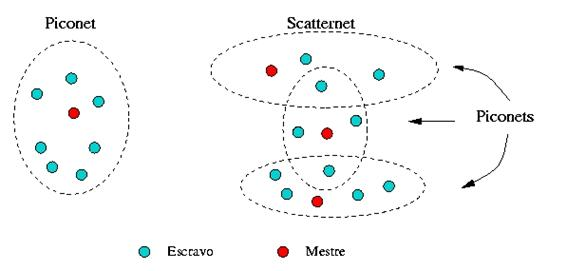
\includegraphics[width=0.6\textwidth]{figuras/scatternet}
    \caption{Redes 802.15 - BlueTooth}
    \label{fig:piconet-scatternet}
\end{figure}

Neste caso, contornar este problema é relativamente fácil. Basta mudar a tecnologia utilizada para comunicação. Esta decisão demanda a implementação de um \emph{driver} específico para esta nova tecnologia escolhida de modo que o SG possa comunicar-se com ela. O protocolo 802.15.4 (\emph{ZigBee Alliance} \cite{zigbee}) é uma solução bem plausível. Sua estrutura permite que em uma rede, comparando-a a uma piconet, haja mais de 50 mil nós com três possíveis topologias (Figura \ref{fig:topologia-zigbee}): estrela, árvore e mesh. A última, em particular, é de extrema elegibilidade, pois é auto adaptável, isto é, quando um nó é removido ou um novo é inserido na rede sua estrutura se reorganiza de modo a não influenciar os demais nós já presentes na rede.

\begin{figure}[htbp]
   \centering
    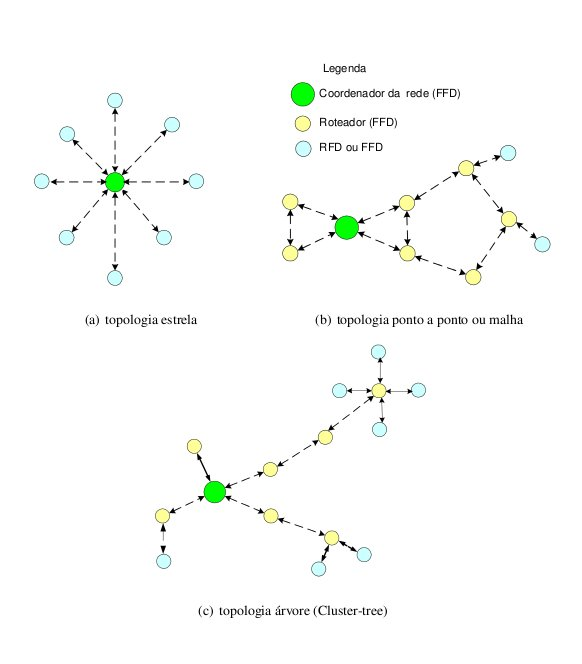
\includegraphics[width=1\textwidth]{figuras/zigbee}
    \caption{Topologias 802.15.4 - ZigBee}
    \label{fig:topologia-zigbee}
\end{figure}

Existem, de fato, diversos pontos que podem ser melhorados, como já foi mostrado. Entretanto, há algumas alterações que demandam uma análise mais profunda e detalhada. Um exemplo bem claro reside no SG utilizado neste protótipo. Este foi desenvolvido em uma linguagem de programação diferente daquela apresentada no trabalho de Trifa\cite{sgtriwiguiboh} gerando uma estrutura diferenciada, como apresentado na Seção \ref{sec:sg}. Um trabalho interessante seria analisar comparativamente qual impacto efetivo que esta mudança trouxe para o sistema como um todo e, principalmente, para o SG, em termos de complexidade de execução, projeto e implementação. Se a estrutura gera alguma fragilidade quanto a não utilização do padrão \emph{Singleton} no projeto, posto que este visa garantir uma instanciação sem ambiguidades do driver.

Ainda há muito a ser feito e as possibilidades são inúmeras, mas este é um grande passo inicial. Espera-se que com este canal aberto, enxergando as possibilidades benéficas que este tipo de trabalho gera, sejam ajudando o público alvo ou a flexibilidade adquirida para a agregação dos conteúdos complexos e desconexos à primeira vista além do conhecimento em si, haja uma expansão da área ou, pelo menos, uma maior procura pelo tema.


%%%%%%%%%%%%%%%%%%%
% parte final
%%%%%%%%%%%%%%%%%%%

\cleardoublepage
\addcontentsline{toc}{chapter}{Referências Bibliográficas}

\begin{thebibliography}{99}
    \bibitem{motrix}
	Projeto Motrix - \url{http://intervox.nce.ufrj.br/motrix/}
    \bibitem{fravisphinx}
	OLIVEIRA, VF,
	\emph{Reconhecimento de Fala Contínua Para O Português Brasileiro Baseado Em HTK e SPHINX}, Projeto Final, Escola Politécnica/COPPE/UFRJ, março 2010

    \bibitem{wotdovad}
	GUINARD, D,
	\emph{Towards the Web of Things: Web Mashups for Embedded Devices}

    \bibitem{wsaniais}
	AKYILDIZ, IF, KASIMOGLU, IH,
	\emph{Wireless Sensor and actor networks: research challenges},
	article, Georgia Institute of Technology/Broadband and Wireless Network Laboratory, maio 2004

    \bibitem{sgtriwiguiboh}
	TRIFA V, WIELAND S, GUINARD D, BOHNERT T,
	\emph{Design and Implementatio of a Gateway for Web-based Interection and Management of Embedded Devices},
	article, Intitut for Pervasive Computing, ETH Zurich, SAP Research CEC Zurich

    \bibitem{rssffla}
	DELICATO, FC,
	\emph{Middleware Baseado em Serviços para Redes de Sensores Sem Fio},
	Dissertação de Doutorado,
	Engenharia Elétrica/COPPE/UFRJ, julho 2005

    \bibitem{restws}
	LEONARDO RICHARDISON, SR,
	\emph{RESTFul Web Serices}, 2007, O'Reilly

    \bibitem{w3curi}
	URI - \url{http://www.w3.org/TR/uri-clarification/}

    \bibitem{w3csoap}
	SOAP - \url{http://www.w3.org/TR/soap}

    \bibitem{w3cxml}
	XML - \url{http://www.w3.org/xml}

    \bibitem{yaml}
	YAML - \url{http://www.yaml.org}

    \bibitem{json}
	JSON - \url{http://www.json.org}

    \bibitem{cmusphinx}
	CMU Sphinx - \url{http://cmusphinx.sourceforge.net}

    \bibitem{restclient}
	Google I/O 2010 - \url{http://www.google.com/events/io/2010/sessions/developing-RESTful-android-apps.html}

    \bibitem{Andy Rubin}
	\url{http://googleblog.blogspot.com/2007/11/wheres-my-gphone.html}

    \bibitem{davis-mermelstein}
	Davis and Mermelstein, 
	\emph{Comparison of Parametric Representations for Monosyllable Word Recognition in Continuously Spoken Sentences},
	IEEE Transactions on Acoustic, Speech and Signal Processing, 1980 .

    \bibitem{Cepstrum}
	Donald G. Childers, David P Skinner, Robert C. Kemerait,
	\emph{The Cepstrum: A Guide to Processing}, 
	Proceedings of the IEEE, VOL. 65, NO. 10, October 1977

    \bibitem{fsr}
	Lawrence Rabiner, Biing-Hwang Juang,
	\emph{Fundamentals of Speech Recognition},
	Pentice-Hall International, Inc, 1993

    \bibitem{arduino}
	Arduino - \url{http://arduino.cc}
    
\bibitem{arduinoapi}
	Linguagem de Programação Arduino - \url{http://arduino.cc/en/Reference/HomePage}

    \bibitem{wiring}
	\emph{Wiring} - \url{http://wiring.org.co/}

    \bibitem{processing}
	\emph{Processing} - \url{http://www.processing.org/}

    \bibitem{Mark Weiser}
	Weiser M.,
	\emph{The Computer of the Twenty-First Century},
	Scientifc America, Vol. 256, No. 3, Sept. 1991, pp. 94-104.

    \bibitem{python}
	\emph{Learning Python},
	
    \bibitem{IoT}
	Dieter Uckelmann, Mark Harrison, Florian Michahelles,
	\emph{Architecting the Internet of Things}
	Springer Science, 2011

\bibitem{swig}
	\emph{SWIG} - \url{http://www.swig.org/}

\bibitem{ndk}
	\emph{Android NDK} - \url{http://developer.android.com/sdk/ndk/index.html}

\bibitem{TCP/IP}
	W. Richard Stevens,
	\emph{The Protocols (TCP/IP Ilustrated Volume I)},
	Addison-Wesley Professional, 1ª edição, Dezembro 1993, ISBN 0-201-63346-9

\bibitem{zigbee}
	\emph{ZigBee Alliance} - \url{http://www.zigbee.org}

\bibitem{bluetooth}
	\emph{Bluetooth SIG} - \url{http://www.bluetooth.com}
\bibitem{recintent}
	\emph{RecognizerIntent} - \url{http://developer.android.com/reference/android/speech/RecognizerIntent.html}

\bibitem{handcent}
	\emph{Handcent SMS} - \url{http://developer.android.com/reference/android/speech/RecognizerIntent.html}
\end{thebibliography}

\end{document}
